\documentclass[10pt,a4paper]{article}
\usepackage[utf8]{inputenc}
\usepackage[T1]{fontenc}
\usepackage[spanish]{babel}
\usepackage{amsmath}
\usepackage{amsfonts}
\usepackage{amssymb}
\usepackage{graphicx}
\usepackage{float}
\usepackage{subcaption}
\usepackage[colorlinks=true, citecolor=blue, final]{hyperref}
\usepackage[table]{xcolor}
\usepackage{amsmath}
\usepackage{graphicx}
\usepackage{epstopdf}

\epstopdfDeclareGraphicsRule{.gif}{png}{.png}{convert gif:#1 png:\OutputFile}
\AppendGraphicsExtensions{.gif}
\usepackage{amssymb}
\setlength{\arrayrulewidth}{1mm}
\setlength{\tabcolsep}{18pt}
\renewcommand{\arraystretch}{2.5}

\usepackage{url} % UTILIZA EL PAQUETE PARA QUE APAREZCA EL URL AUNQUE AUN NOSE SI DEBO ACTIVARLO TAMBIEN EN REFERENCIAS
\hypersetup{
    colorlinks=true,
    linkcolor=blue,
    filecolor=blue,      
    urlcolor=blue,
}
\usepackage{epsfig}
\hypersetup{colorlinks=true,
    linkcolor=blue,
    filecolor=blue,      
    urlcolor=blue,}

\usepackage{graphicx}
\usepackage[sort&compress, numbers]{natbib}
\usepackage{xcolor}
\usepackage{listings}
\usepackage{ragged2e}
\definecolor{codegreen}{rgb}{0,0.6,0}
\definecolor{codegray}{rgb}{0.5,0.5,0.5}
\definecolor{codepurple}{rgb}{0.58,1,0.82}
\definecolor{backcolour}{rgb}{1,1,0.97}
\lstdefinestyle{mystyle}{
    backgroundcolor=\color{backcolour},   
    commentstyle=\color{codegreen},
    keywordstyle=\color{magenta},
    numberstyle=\tiny\color{codegray},
    stringstyle=\color{codepurple},
    basicstyle=\ttfamily\footnotesize,
    breakatwhitespace=false,         
    breaklines=true,                 
    captionpos=b,                    
    keepspaces=true,                 
    numbers=left,                    
    numbersep=5pt,                  
    showspaces=false,                
    showstringspaces=false,
    showtabs=false,                  
    tabsize=2
}
\lstset{style=mystyle}
\usepackage{lipsum}
\usepackage{multicol}
\usepackage{xcolor}
\newcommand{\celda}[1]{
	\begin{minipage}{2cm}
		\vspace{2mm}
		#1
		\vspace{2mm}
	\end{minipage}
}
\definecolor{azul}{rgb}{0.36, 0.54, 0.66}
\usepackage[left=2.00cm, right=2.00cm, top=2.00cm, bottom=2.00cm]{geometry}
\author{Jorge Vicente Niño Mocarro}
\begin{document}
	
	\begin{figure}[H]
		\raggedright
		\includegraphics[scale=0.5]{uanl.png} \hfill \includegraphics[scale=0.275]{fime.png}
	\end{figure}

	\vspace{6mm}
	
	%ESTE CENTER ES EXCLUSIVO PARA EL TITULO DEL PAPER, AUTOR Y UNIVER.
	\begin{center}
		{\Large \textbf{Práctica 9: Interacciones entre partículas}}\\
		\vspace{2mm}
		\textit{ Alumno: José Adrian Garcia Fuentes}\\
		\textit{Profesor: Satu Elisa Schaeffer.}\\
		\vspace{2.5mm}
		\textit{Universidad Autónoma de Nuevo León. Facultad de Ingeniería Mecánica y Eléctrica.}\\
		\vspace{1mm}
		\textit {25/abril/2021 }
		
		
	\end{center}

	\begin{center}
		\textcolor{azul}{\rule{150mm}{0.8mm}}
	\end{center}

      %ESTE ABSTRACT ES PARA EL RESUMEN PROPIAMENTE DICHO Y PARA LAS PALABRAS CLAVES (KEYWORDS) ,NOTA:el comando \par sirve para iniciar el nuevo parrafo con sangría.
	\begin{abstract}
		En esta práctica se analizará un modelo de atracción y repulsión de partículas con carga. Cada una de estas partículas tiene una propiedad inicial. El principal objetivo es agregar una nueva propiedad llamada masa. Esto permite que se pueda agregar por medio de ecuaciones el comportamiento que ejerce las fuerzas electrostáticas. En cierta distancia las partículas pueden ser atraídas por una fuerza, pero también mantienen su propia masa constante, lo que significa que presentan repulsión a cierta medida.
		\vspace{2mm}\par
		\underline{\textbf{Palabras Claves:}} \hspace{2mm} \textit{atracción, repulsión.}
	\end{abstract}
	
	\begin{center}
		\textcolor{azul}{\rule{150mm}{0.8mm}}
	\end{center}
	
	\vspace{5mm}

	\begin{multicols}{2}
		\section{Introducción} \label{Intro}
		En la práctica 9 se detallan las instrucciones y códigos para simular una interacción entre partículas con carga en un espacio bidimensional. Estas partículas siguen leyes de atracción similares a las expresadas por la ley de Coulomb, moviéndose en una dirección que depende de la interacción de cargas presentes en el sistema y con una fuerza directamente proporcional a la diferencia de cargas e inversamente proporcional a la distancia que las separa. Supongamos que contemos con partículas que habitan un cuadro unitario bidimensional y que cada partícula tiene una carga eléctrica, distribuida independiente y normalmente al azar entre [$-1,1$]. Cargas de un mismo signo producirán una repulsión mientras cargas opuestas resultan en una atracción, la magnitud de la fuerza estará proporcional a la diferencia de magnitud de las cargas (mayores diferencias resultando en fuerzas mayores), y además la fuerza será inversamente proporcional a la distancia euclidiana entre las partículas. Vamos a comenzar creando y posicionando las partículas, usando la distribución normal para las coordenadas 
$x$
y 
$y$
. Ahora, cada partícula va a ejercer una fuerza sobre cada otra partícula. Vamos a implementar la atracción entre cargas con signos opuestos y la repulsión entre signos iguales. Habrá que sumar los efectos de todas las fuerzas individuales para determinar la fuerza total sobre una partícula en específico. Luego debemos normalizar el efecto de esa fuerza con un factor de descuento antes de poder trasladar la partícula con desplazamientos y que dependen de los 
componentes horizontales
y vertical de la fuerza total \cite{p9}.
		\section{Objetivo} \label{antece}
		\begin{itemize}
		
		    \item Agregar a cada partícula una masa y que la masa afecte a la velocidad de movimiento \cite{p9}.
		    \item La masa agregada causara una fuerza de atraccion a otra masa \cite{p9}.
		    \item Graficar los $3$ factores Magnitud de carga, Velocidad, y Masa de partículas \cite{p9}.
		    \item Agregar reto 1 en donde las partículas más grandes absorban a las más pequeñas en caso de quedar entre dos de ellas \cite{p9}.
		    \item Agregar reto 2 con diferencia de sobreposición en las partículas \cite{p9}.
		\end{itemize}
	\section{Metodologia}	
	La metodología empleada se realizó a través de Rstudio \cite{RStudio} llevando a cabo los pasos señalados en la \textit{Práctica 9: Interacciones entre partículas} \cite{p9}, a partir del código en el repositorio de Schaeffer \cite{GITSCHAEFFER}, se realizaron modificaciones. El código completo de la metodología empleada se encuentra en el repositorio de GitHub \cite{gitadrian} donde también se pueden encontrar los archivos .Gif de los retos.
	\section{Resultados}
	En esta práctica se tienen una cantidad $n$ de partículas en un cuadro unitario, cada una de ellas posee una carga y una masa. El objetivo es verificar gráficamente que existe una relación entre los factores velocidad, carga y masa de partículas. Las partículas son posicionadas normalmente al azar en el cuadro unitario tal como se muestra en la figura \ref{fig.1}. 
				\begin{figure}[H]
				\centering
				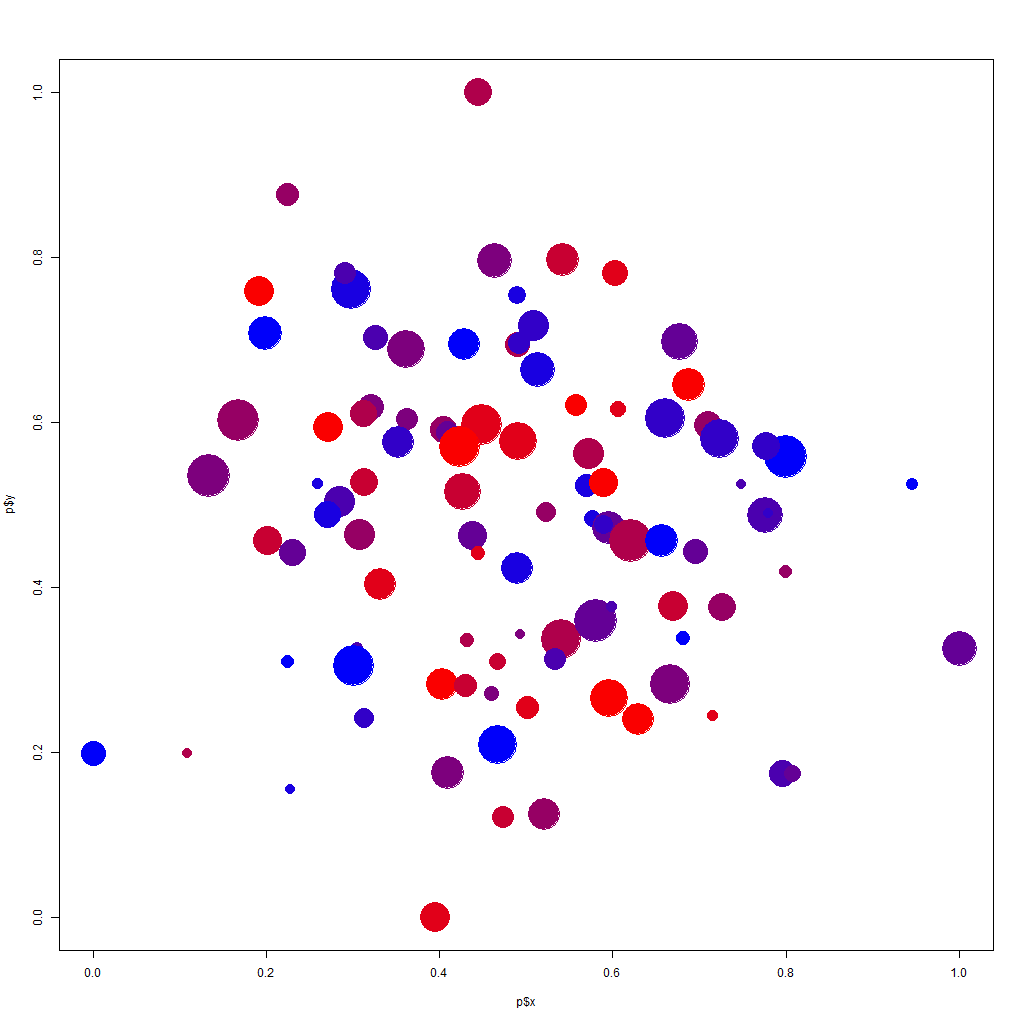
\includegraphics[scale=0.2]{p9i.png}
				\caption{Partículas Carga, Masa, Velocidad.}
				\label{fig.1}
			\end{figure}
	Además, éstas posen una carga que causa fuerzas de repulsión y atracción con las demás partículas si dos partículas tienen el mismo signo o diferente, respectivamente. Se desea añadir otro atributo a las partículas que afecte dicha interacción, este atributo es la masa. Se muestra la interacción entre partículas, el atributo de la masa es representado con círculos de diferente tamaño para mostrar las diferencias entre las masas de las partículas. Esta interacción se puede apreciar de una mejor manera en una animación \cite{gitadrian}. Toda la información se almacena en un data.frame, del cual se muestra un fragmento en el cuadro \ref{tb: Tabla1} para observar los datos obtenidos de cada partícula ver el apartado de factores en el repositorio de github \cite{gitadrian}.
	
	
			\begin{figure}[H]
				\centering
				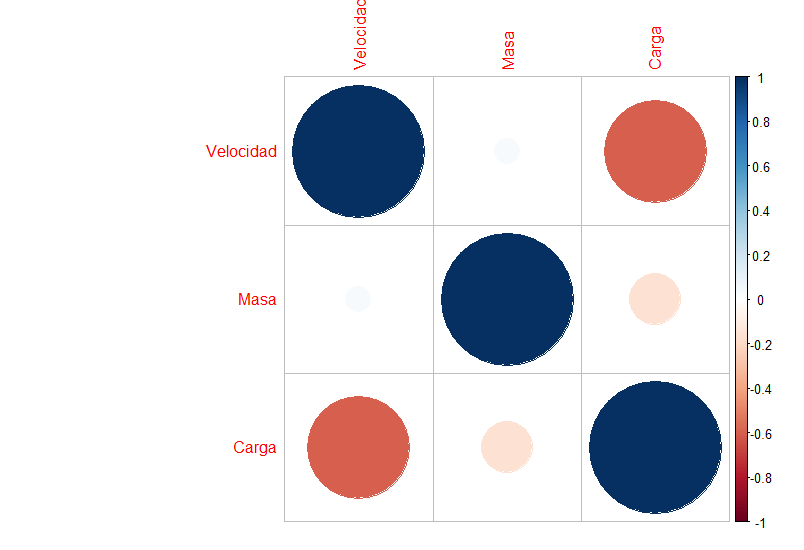
\includegraphics[scale=0.4]{Rplot.png}
				\caption{Gráfico corrplot Velocidad, Masa, Carga.}
				\label{fig: Figura1}
			\end{figure}
				Con la información obtenida, se realizan diversos gráficos los factores: velocidad, masa y carga. La figura \ref{fig: Figura1} muestra dichos gráficos y como se aprecia la carga y la masa afectan a la velocidad y su relación se muestra en el cuadro \ref{tb: Tabla2}. En la figura \ref{fig.3} se muestran las partículas con masa mas grande que absorben alas demás cuando se colocan entre dos partículas y en la figura \ref{fig.4} las partículas interactúan entre si, sin sobreponerse. \\

		Observe los archivos .gifs en el repositorio de GitHub \cite{gitadrian}.
					\begin{figure}[H]
				\centering
				\includegraphics[scale=0.4]{SOBREPOSISCION.png}
				\caption{Partículas Carga, Masa, Velocidad(Reto 1).}
				\label{fig.3}
			\end{figure}
				\begin{figure}[H]
				\centering
				\includegraphics[scale=1]{ELIMINACION.png}
				\caption{Partículas Carga, Masa, Velocidad(Reto 2).}
				\label{fig.4}
			\end{figure}



\end{multicols}
	\begin{table}[H]
		\centering
		\caption{Fuerzas de las $n$ partículas.}
		\begin{tabular}{cccc}
			\hline
			 \celda{Velocidad} & \celda{Masa} & \celda{Carga}\\
			\hline
			\celda{$0.01$} & \celda{$0.96$} & \celda{$0.02$} \\
			\hline
			\celda{0.00} & \celda{0.97} & \celda{0.20}\\
			\hline
		\end{tabular}
	\label{tb: Tabla1}
	\end{table}
	\begin{multicols}{2}

			
\newpage
\begin{lstlisting}
n <- 50
p <- data.frame(x = rnorm(n), y=rnorm(n), c=rnorm(n), m=runif(n,min=.001, max=1))
xmax <- max(p$x)
xmin <- min(p$x)
p$x <- (p$x - xmin) / (xmax - xmin) 
ymax <- max(p$y)
ymin <- min(p$y)
p$y <- (p$y - ymin) / (ymax - ymin) 
cmax <- max(p$c)
cmin <- min(p$c)
p$c <- 2 * (p$c - cmin) / (cmax - cmin) - 1 
p$g <- round(5 * p$c) 
paso <- floor(256 / 10)
niveles <- seq(0, 255, paso)
colores <- rgb(niveles, rep(0, 11), rev(niveles), max=255)
eps <- 0.001
fuerza <- function(i) {
  xi <- p[i,]$x
  yi <- p[i,]$y
  ci <- p[i,]$c
  mi <- p[i,]$m
  fx <- 0
  fy <- 0
  for (j in 1:n) {
    cj <- p[j,]$c
    mj <- p[j,]$m
    dir <- (-1)^(1 + 1 * (ci * cj < 0))
    dx <- xi - p[j,]$x
    dy <- yi - p[j,]$y
    if (dir>0) {
      factor <- dir * abs(ci - cj) * ((1+mi * (1+mj)^3)^(1/8)) / (sqrt(dx^2 + dy^2) + eps)
    } else {
      factor <- dir * abs(ci - cj) / (sqrt(dx^2 + dy^2) + eps)
    }
    fx <- fx - dx * factor
    fy <- fy - dy * factor
  }
  return(c(fx, fy))
}
suppressMessages(library(doParallel))
registerDoParallel(makeCluster(detectCores() - 1))
tmax <- 100
digitos <- floor(log(tmax, 10)) + 1
tl <- "0"
while (nchar(tl) < digitos) {
  tl <- paste("0", tl, sep="")
}
plot(p$x, p$y, col=colores[p$g+6], pch=15, cex=1.5, xlim=c(-0.1, 1.1), ylim=c(-0.1, 1.1),
     main="Estado inicial", xlab="X", ylab="Y")
f.iter=matrix(ncol=tmax, nrow=n*2)
for (iter in 1:tmax) {
  f <- foreach(i = 1:n, .combine=c) %dopar% fuerza(i)
  delta <- 0.02 / max(abs(f)) 
  p$x <- foreach(i = 1:n, .combine=c) %dopar% max(min(p[i,]$x + delta * f[c(TRUE, FALSE)][i], 1), 0)
  p$y <- foreach(i = 1:n, .combine=c) %dopar% max(min(p[i,]$y + delta * f[c(FALSE, TRUE)][i], 1), 0)
  for(i in 1:(n*2)) { f.iter[i,iter] <- f[i] * delta }
  tl <- paste(iter, "", sep="")
  while (nchar(tl) < digitos) {
    tl <- paste("0", tl, sep="")
  }
  plot(p$x, p$y, col=colores[p$g+6], pch=15, cex=1.5, xlim=c(-0.1, 1.1), ylim=c(-0.1, 1.1),
       main=paste("Paso", iter), xlab="X", ylab="Y")
}
stopImplicitCluster()
f.iter.distance=matrix(ncol=tmax, nrow=n)
f.iter.media ="0"
for (t in 1:tmax) {
  for (i in 1:n) {
    k = i*2
    f.iter.distance[i,t] <- sqrt(f.iter[k,t]^2 + f.iter[k-1,t]^2)
  }
}
for (i in 1:n) {
  p$v[i]<-mean(f.iter.distance[i,])
}
factores<-cbind(p$v,p$m, p$c)
colnames(factores) <- c("Velocidad","Masa", "Carga")
corrplot(cor(factores) )
	\end{lstlisting}
\end{multicols}		
	
	\begin{table}[H]
		\centering
		\caption{Relación de fuerzas.}
		\begin{tabular}{cccc}
			\hline
			\celda{} & \celda{Velocidad} & \celda{Masa} & \celda{Carga}\\
			\hline
			\celda{Velocidad} & \celda{$1.0$} & \celda{$0.213$} & \celda{$0.13$}\\
			\hline
			\celda{Masa} & \celda{$0.213$} & \celda{$1.0$} & \celda{$0.10$}\\
			\hline
			\celda{Carga} & \celda{$0.13$} & \celda{$0.10$} & \celda{$1.0$}\\
			\hline
		\end{tabular}
		\label{tb: Tabla2}
	\end{table}
	\vspace{5mm}
	\begin{multicols}
\\	\section{Conclusión}
	
La interacción entre partículas con carga y agregando propiedades como la masa pueden afectar directamente el movimiento en la dirección y la velocidad de otras ya que a una mayor masa las partículas tenderán a moverse lentamente debido a su peso pero su fuerza electrostática o fuerza de atracción repulsión será mayor en caso contrario como se ve en las partículas más pequeñas muchas tenderán a moverse más rápidamente para el caso del reto 1 se puede tomar como una reacción de aglomeración en que al sobreponerse o pasar muy cerca de partículas de mayor tamaño estas tenderán a unirse a el caso contrario en el reto dos en el que no existe una superposición a la partícula de mayor masa.

\bibliography{T9}
	\end{multicols}
\bibliographystyle{ieeetr}
	
\end{document}